\documentclass[a4paper, 11pt]{article}
\usepackage[margin=3cm]{geometry}
\usepackage[]{fontenc}
\usepackage[utf8]{inputenc}
\usepackage[italian]{babel}
\usepackage{geometry}
\usepackage{amsmath}
\usepackage{amssymb}
\usepackage{gensymb}
\usepackage{graphicx}
\usepackage{psfrag,amsmath,amsfonts,verbatim}
\usepackage{xcolor}
\usepackage{color,soul}
\usepackage{fancyhdr}
\usepackage{indentfirst}
\usepackage{graphicx}
\usepackage{newlfont}
\usepackage{amssymb}
\usepackage{amsmath}
\usepackage{latexsym}
\usepackage{amsthm}
\usepackage{subfigure}
\usepackage{subcaption}
\usepackage{psfrag}
\usepackage{footnote}
\usepackage{graphics}
\usepackage{color}
\usepackage{hyperref}
\usepackage{tikz}
\usepackage{float}

\usetikzlibrary{snakes}
\usetikzlibrary{positioning}
\usetikzlibrary{shapes,arrows}

	
	\tikzstyle{block} = [draw, fill=white, rectangle, 
	minimum height=3em, minimum width=6em]
	\tikzstyle{sum} = [draw, fill=white, circle, node distance=1cm]
	\tikzstyle{input} = [coordinate]
	\tikzstyle{output} = [coordinate]
	\tikzstyle{pinstyle} = [pin edge={to-,thin,black}]

\newcommand{\courseacronym}{CAT}
\newcommand{\coursename}{Controlli Automatici - T}
\newcommand{\tipology}{B}
\newcommand{\trace}{1}
\newcommand{\projectname}{Controllo di una tavola rotante motorizzata}
\newcommand{\group}{49}

%opening
\title{ \vspace{-1in}
		\huge \strut \coursename \strut 
		\\
		\Large  \strut Progetto Tipologia \tipology - Traccia \trace 
		\\
		\Large  \strut \projectname\strut
		\\
		\Large  \strut Gruppo \group\strut
		\vspace{-0.4cm}
}
\author{ Isacco Briali, Emanuele Coacci, Davide Gianessi}
\date{}

\begin{document}

\maketitle
\vspace{-0.5cm}
In questo progetto studiamo il controllo di una tavola rotante motorizzata, collegata ad un motore tramite un giunto cardanico. La dinamica del sistema è descritta dalle seguenti equazioni differenziali:
%
\begin{subequations}\label{eq:system}
\begin{align}
	    J\dot{w} &= \tau(\theta)C_m - \beta\omega - k\theta,
        \\
        dove \hspace{0,2cm} \spac \tau(\theta) &= \frac{\cos{\alpha}}{1-(\sin{\alpha\cos{\theta)^2}}}
\end{align}
\end{subequations}
%

Assumiamo $\theta$(t) la posizione angolare della tavola e $\omega$(t) la sua velocità angolare. Otteniamo dal sistema scritto in precedenza che $\tau$($\theta$) è il rapporto di trasmissione del giunto cardanico funzione $\theta$ e dell'angolo tra i due alberi $\alpha$, mentre J è il momento di inerzia della tavola. Completando le equazioni abbiamo $C_m$ come imput di controllo, ossia la coppia generata dal motore elettrico, e i due coeficienti $\beta$ e k che sono rispettivamente l'attrito viscoso e l'elasticità del disco. Supponiamo in oltre che la posizione angolare $\theta$ della tavola possa essere misurata.

Per la realizzazzione di questo progetto, per maggiore comodità, usabilità ed efficienza, abbiamo adoperato due diversi ambienti: Python e MATLAB. Con il primo abbiamo effettuato tutti i calcoli che verranno riportati in seguito nella relazione e il test sul sistema lineare. Il secondo, invece, lo abbiamo utilizzato per effettuare i test del regolatore sia sul sistema lineare, sia sul sistema non lineare.

\section{Espressione del sistema in forma di stato e calcolo del sistema linearizzato intorno ad una coppia di equilibrio}

Innanzitutto, esprimiamo il sistema~\eqref{eq:system} nella seguente forma di stato
%
\begin{subequations}
\begin{align}\label{eq:state_form}
	\dot{x} &= f(x,u)
	\\
	y &= h(x,u).
\end{align}
\end{subequations}
%
Pertanto, andiamo a individuare lo stato $x$, l'ingresso $u$ e l'uscita $y$ del sistema come segue 
%
\begin{align*}
x := \begin{bmatrix}
	    x_1\\
            x_2     
	\end{bmatrix} := \begin{bmatrix}
	    \theta\\
        \omega     
	\end{bmatrix}, \quad u := C_m, \quad y := \theta.
\end{align*}
%
Coerentemente con questa scelta, ricaviamo dal sistema~\eqref{eq:system} la seguente espressione per le funzioni $f$ ed $h$
%
\begin{align*}
	f(x,u) &:= \begin{bmatrix}
	    f_1(x,u)\\
            f_2(x,u)     
	\end{bmatrix} := \begin{bmatrix}
	    x2\\
            \frac{\frac{\cos{\alpha}}{1-(\sin{\alpha}\cos{x_1})^2}C_m - \beta x_2 - kx_1}{J}     
	\end{bmatrix}
	\\
	h(x,u) &:= x_1.
\end{align*}
%
Una volta calcolate $f$ ed $h$ esprimiamo~\eqref{eq:system} nella seguente forma di stato
%
\begin{subequations}\label{eq:our_system_state_form}
\begin{align}
	\begin{bmatrix}
		\dot{x}_1
		\\
		\dot{x}_2
	\end{bmatrix} &= \begin{bmatrix}
	    x2\\
            \frac{\frac{\cos{\alpha}}{1-(\sin{\alpha}\cos{x_1})^2}C_m - \beta x_2 - kx_1}{J}     \end{bmatrix} \label{eq:state_form_1}
	\\
	y &= x_1.
\end{align}
\end{subequations}
%
Da specifiche ci viene dato il valore di equilibrio $ x_e = \begin{bmatrix}
		x_{1,e}
		\\
		x_{2,e}
	\end{bmatrix} = 
    \begin{bmatrix}
		\theta_e
		\\
		\omega_e
	\end{bmatrix} =
 \begin{bmatrix}
		120^\circ
		\\
		0
	\end{bmatrix}$

A partire dal quale troviamo la coppia di equilibrio $(x_e, u_e)$ di~\eqref{eq:our_system_state_form}, risolvendo il seguente sistema di equazioni
%
\begin{align}
	\begin{bmatrix}
		\dot{x}_1
		\\
		\dot{x}_2
	\end{bmatrix} = \begin{bmatrix}
		0
		\\
		0
	\end{bmatrix} = \begin{bmatrix}
		0
		\\
		\frac{\sqrt{3}u-125\pi}{1500}
	\end{bmatrix}
\end{align}
%
dal quale otteniamo
%
\begin{align}
	x_e := \begin{bmatrix}
		120^\circ
		\\
		0
	\end{bmatrix},  \quad u_e = 226.7249\label{eq:equilibirum_pair}
\end{align}
%
Definiamo le variabili alle variazioni $\delta x$, $\delta u$ e $\delta y$ come 
%
\begin{align*}
	\delta x &= x-x_e, 
	\quad
	\delta u = u-u_e, 
	\quad
	\delta y = y-y_e.
\end{align*}
%
L'evoluzione del sistema espressa nelle variabili alle variazioni pu\`o essere approssimativamente descritta mediante il seguente sistema lineare
%
\begin{subequations}\label{eq:linearized_system}
\begin{align}
	\delta \dot{x} &= A\delta x + B\delta u
	\\
	\delta y &= C\delta x + D\delta u,
\end{align}
\end{subequations}
%
dove le matrici $A$, $B$, $C$ e $D$ vengono calcolate come
%
\begin{subequations}\label{eq:matrices}
\begin{align}
	A &= \begin{bmatrix}
		\frac{\partial f_1(x,u)}{\partial x_1} & \frac{\partial f_1(x,u)}{\partial x_2}
		\\
		\frac{\partial f_2(x,u)}{\partial x_1} & \frac{\partial f_2(x,u)}{\partial x_2}
	\end{bmatrix}_{\substack{x = x_e\\u = u_e}} = \begin{bmatrix}
		  0 & 1
		\\
		-0.06454 & -0.00075
	\end{bmatrix}
	\\
	B &= \begin{bmatrix}
		\frac{\partial f_1(x,u)}{\partial u}
		\\
		\frac{\partial f_2(x,u)}{\partial u}
	\end{bmatrix}_{\substack{x = x_e\\u = u_e}} = \begin{bmatrix}
	       0 \\ 0.001154
	\end{bmatrix}
	\\
	C &= \begin{bmatrix}
		\frac{\partial h(x,u)}{\partial x_1}
		&
		\frac{\partial h(x,u)}{\partial x_2}
	\end{bmatrix}_{\substack{x = x_e\\u = u_e}} = \begin{bmatrix}
	    1 & 0
	\end{bmatrix}
	\\
	D &= \begin{bmatrix}
		\frac{\partial h(x,u)}{\partial u}
	\end{bmatrix}_{\substack{x = x_e\\u = u_e}} = \begin{bmatrix}
	    0
	\end{bmatrix}
\end{align}
\end{subequations}
%
\section{Calcolo Funzione di Trasferimento}

In questa sezione, andiamo a calcolare la funzione di trasferimento $G(s)$ dall'ingresso $\delta u$ all'uscita $\delta y$ mediante la seguente formula 
%
%
\begin{align}\label{eq:transfer_function}
G(s) = C(sI -A)^{-1} B+D = \frac{0.0011547}{s^2+0.00075s+0.18546}.
\end{align}

Dunque il sistema linearizzato~\eqref{eq:linearized_system} è caratterizzato dalla funzione di trasferimento~\eqref{eq:transfer_function} con $2$ poli complessi coniugati $p_1p_2 = -0.000375 \pm 0.254j $ e uno\\ In Figura ~\ref{Figura1} mostriamo il corrispondente diagramma di Bode. 
\begin{figure}[H]
    \centering
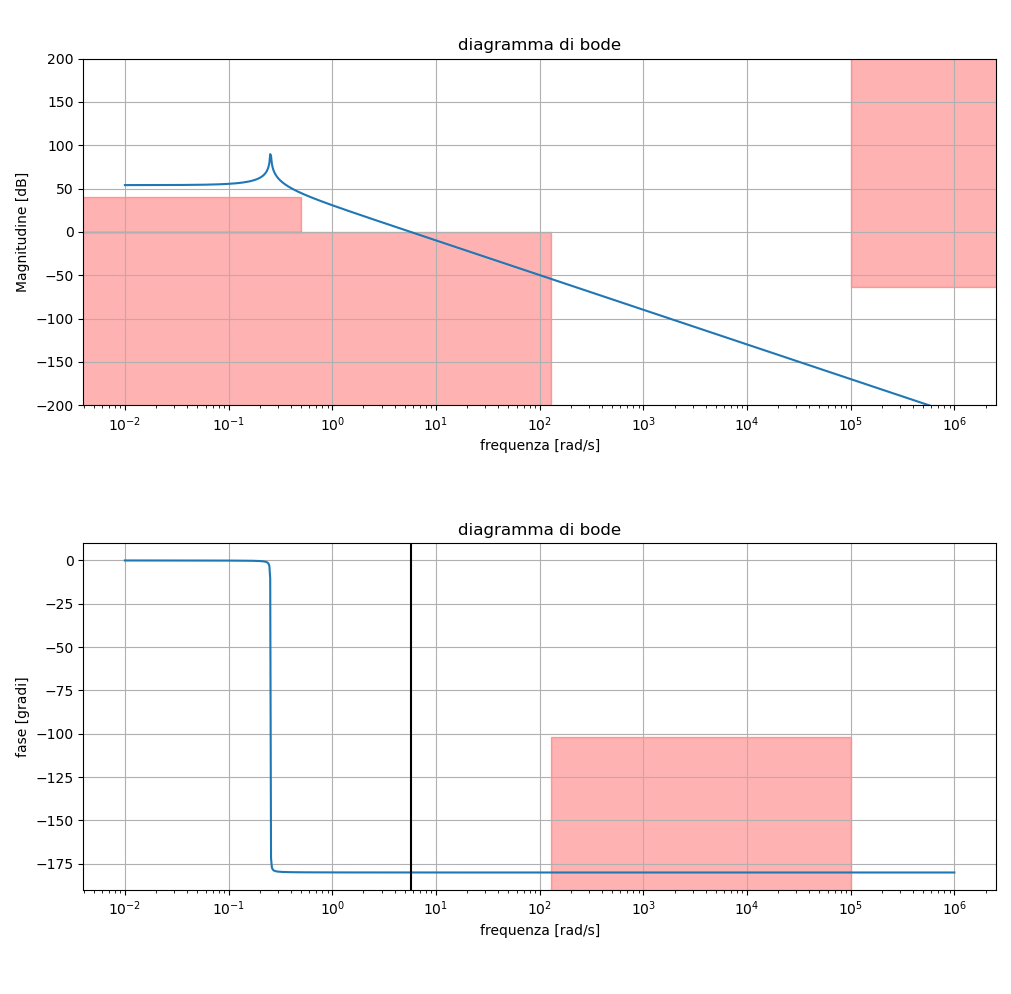
\includegraphics[width=110mm]{figs/bode_G.png}
    \caption{}
    \label{Figura1}
\end{figure}

\section{Mappatura specifiche del regolatore}
\label{sec:specifications}

Le specifiche da soddisfare sono
\begin{itemize}
	\item[1)] Errore a regime $\space |e_{\infty}| \le e^* = 0.005 $ con riferimeto a gradino
	\\
	\item[2)] $M_f \ge 30\degree$ 
 \\
	\item[3)] $S\%\ge 2\%$: ovvero $M_f \ge 77.97\degree$
 \\
	\item[4)] $T_{a,5} = 0.03s$. 
 \\
	\item[5)]$d(t)$ attenuato di almeno $40dB$ in $\begin{bmatrix}
	    0 , & 0.5
	\end{bmatrix}$
 \\
	\item[6)]$n(t)$ attenuato di almeno $63dB$ in $\begin{bmatrix}
	    10^5 , & 10^6
	\end{bmatrix}$
\end{itemize}
%
Andiamo ad effettuare la mappatura punto per punto le specifiche richieste.

\begin{itemize}
	\item[1)] L'errore a reggime $e_{\infty}$ $ < $ 0.005 in risposta a un gradino w(t) = 1(t) e d(t) = 1 (t) .\\
	\item[2)] Le specifiche 2 e 3 sono entrambe sul margine di fase, perci\`o andiamo a soddisfare la pi\`u stringente. Otteniamo quindi $M_f\ge77.97\degree$.
	\\
	\item[3)] Dalla specifica 4, sul tempo di assestamento $T_{a,5}$, ricaviamo: $\omega _c \ge \frac{300}{0,03 M_f} \approx 128.25$rad/s.
	\item[4)] Dalla specifica 5 ricaviamo $|L(j\omega)|_{dB} \ge 40dB$ in $\begin{bmatrix}
	    0 , & 0.5
	\end{bmatrix}$.\\
	\item[5)] Dalla specifica 6 ricaviamo $|L(j\omega)|_{dB} \le -63dB$ in$\begin{bmatrix}
	    10^5 , & 10^6
	\end{bmatrix}$.\\
\end{itemize}

Pertanto, in Figura ~\ref{Figura2}, mostriamo il diagramma di Bode della funzione di trasferimento $G(s)$ con le zone proibite emerse dalla mappatura delle specifiche.
\begin{figure}[H]
    \centering
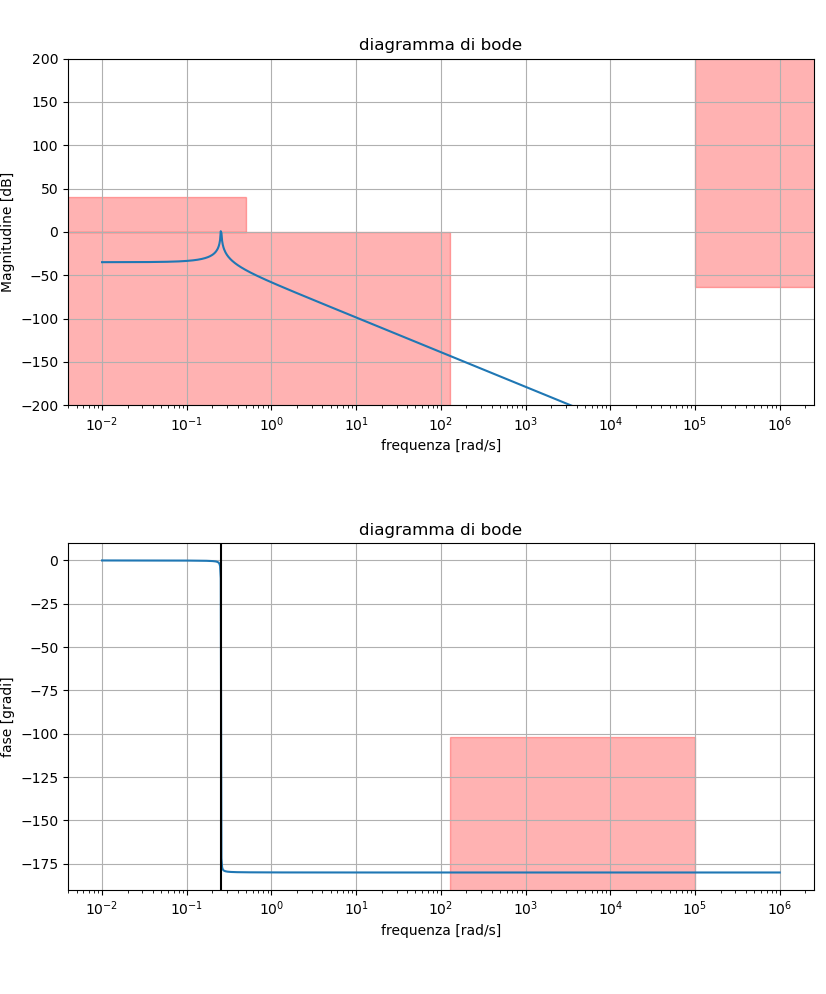
\includegraphics[width=110mm]{figs/bode_G_mapping.png}
    \caption{}
    \label{Figura2}
\end{figure}
\section{Sintesi del regolatore statico}
\label{sec:static_regulator}

In questa sezione progettiamo il regolatore statico $R_s(s)$ partendo dalle analisi fatte in sezione~\ref{sec:specifications}.
Per ridurre l'errore a regime del sistema aumentiamo il guadagno statico $\mu$ del regolatore in modo tale da portare $e_\infty \space $ sotto 0.005.

Dunque, definiamo la funzione estesa $G_e(s) = R_s(s)G(s)$ e, in Figura ~\ref{Figura3}, mostriamo il suo diagramma di Bode per verificare se e quali zone proibite vengono attraversate.
\begin{figure}[H]
    \centering
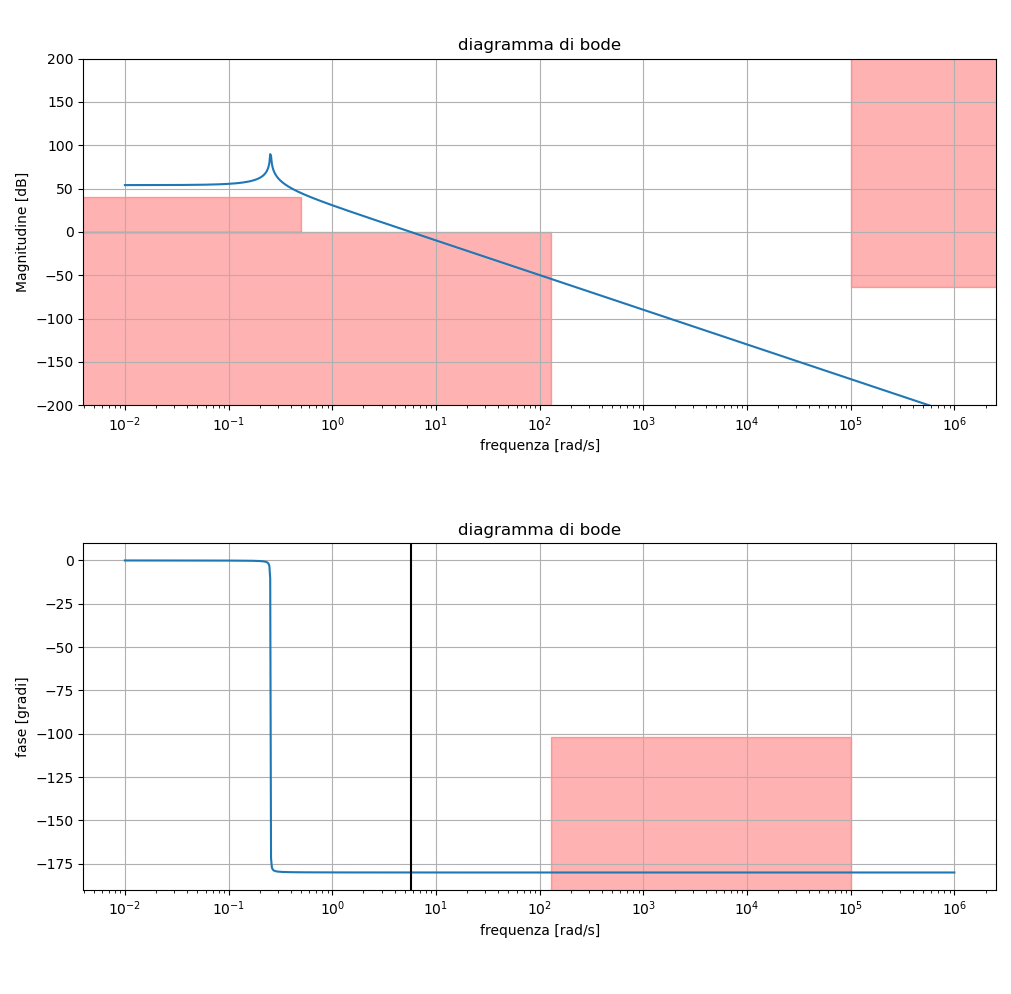
\includegraphics[width=110mm]{figs/bode_Ge.png}
    \caption{}
    \label{Figura3}
\end{figure}
Da Figura ~\ref{Figura3}, emerge che la $G_e(s)$ non rispetta i vincoli sul margine di fase $M_f$ e sul tempo di assestamento $\omega_{c,min}$


\section{Sintesi del regolatore dinamico}

In questa sezione, progettiamo il regolatore dinamico $R_d(s)$. 
%
Dalle analisi fatte in Sezione~\ref{sec:static_regulator}, notiamo di essere nello Scenario di tipo B. Dunque, progettiamo $R_d(s)$ riccorrendo ad una rete anticipatrice. Utilizziamo le formule di inversione per calcolare $\alpha$ e $\tau$ di $R_d(s)$, prendendo $M_f^*=M_{f,spec}+10$ e $\omega_c=256.51$. Otteniamo quindi:

\begin{align}\label{eq:R_s}
R_s(s)=\frac{1+\tau s}{1+\tau\alpha s}
\end{align}

In Figura ~\ref{Figura4}, mostriamo il diagramma di Bode della funzione d'anello $L(s) = R_d(s) G_e(s)$
\begin{figure}[H]
    \centering
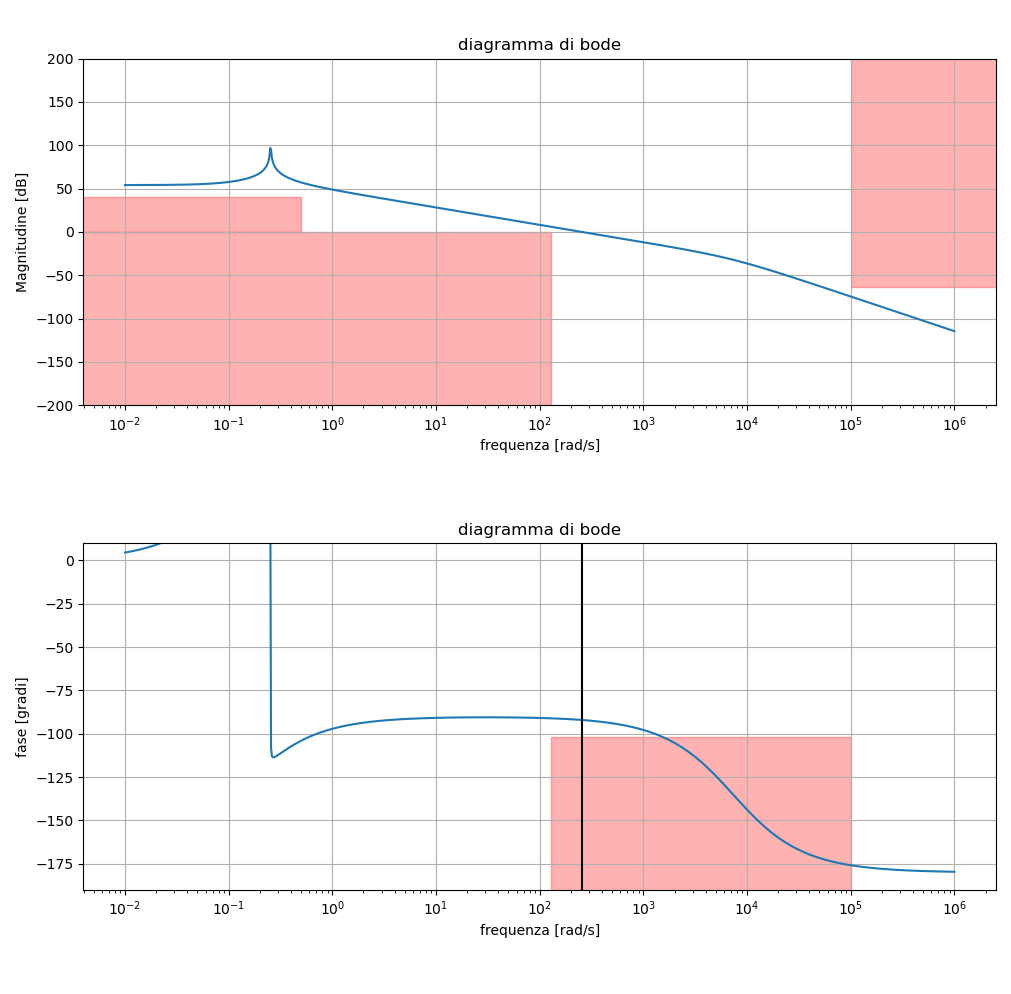
\includegraphics[width=110mm]{figs/bode_L.png}
    \caption{}
    \label{Figura4}
\end{figure}
\section{Test sul sistema linearizzato}

In questa sezione, testiamo l'efficacia del controllore progettato sul sistema linearizzato considerando in primo luogo le risposte al riferimento a gradino w(t) e ai rumori $n(t)$ e $d(t)$, per poi ottenere l'uscita complessiva $y_{\text{tot}}$ sommando le singole risposte per il princio di sovrapposizione degli effetti. Specifichiamo inoltre che, come detto all'inizio, il test è stato effettuato sia su MATLAB che su python; mostriamo in seguito il grafico realizzato con Python.

%
\begin{subequations}\label{eq:system}
\begin{align}
	    y_w &= F(s)W(s)
        \\
        y_d &= S(s)D(s)
        \\
        y_n &= -F(s)N(s)
        \\
        y_{\text{tot}}&= y_w+y_d+y_n
\end{align}
\end{subequations}
%
\begin{figure}[H]
    \centering
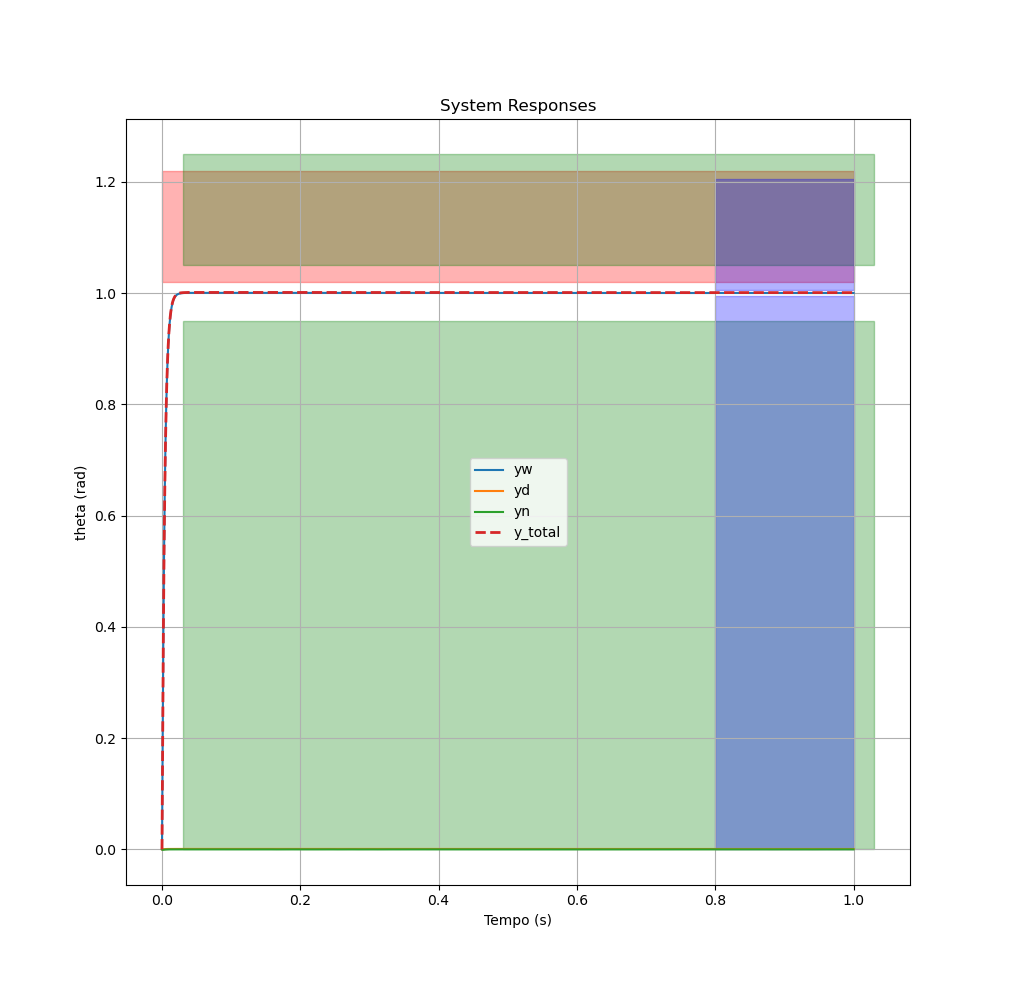
\includegraphics[width=110mm]{figs/linear_sim.png}
    \caption{}
    \label{Figura6}
\end{figure}


Da Figura 5 notiamo che l'uscita soddisfa i vincoli relativi alla sovraelongazione percentuale, al tempo di assestamento e all'errore a regime.

\section{Test sul sistema non lineare}

In questa sezione, testiamo l'efficacia del controllore progettato sul modello non lineare.


Per fare ciò useremo l'estensione simulink di MATLAB. Per poter testare il regolatore sul sistema non lineare dobbiamo effettuare due operazioni:

\begin{itemize}
	\item[1)] Aggiungere $u_e$ in ingresso al sistema come parte dell'ingresso totale $u$, quindi $u = \delta u + u_e$. L'uscita sarà $y$ anziché $\delta y$.
 \\
        \item[2)]Sottrarre $y_e$ in uscita al sistema, così da avere l'uscita $\delta y = y - y_e$. Questo consentirà di calcolare l'errore $e$ sottraendo $\delta y$ dal riferimento w e utilizzarlo come ingresso per il regolatore.
\end{itemize}

\begin{figure}[H]
    \centering
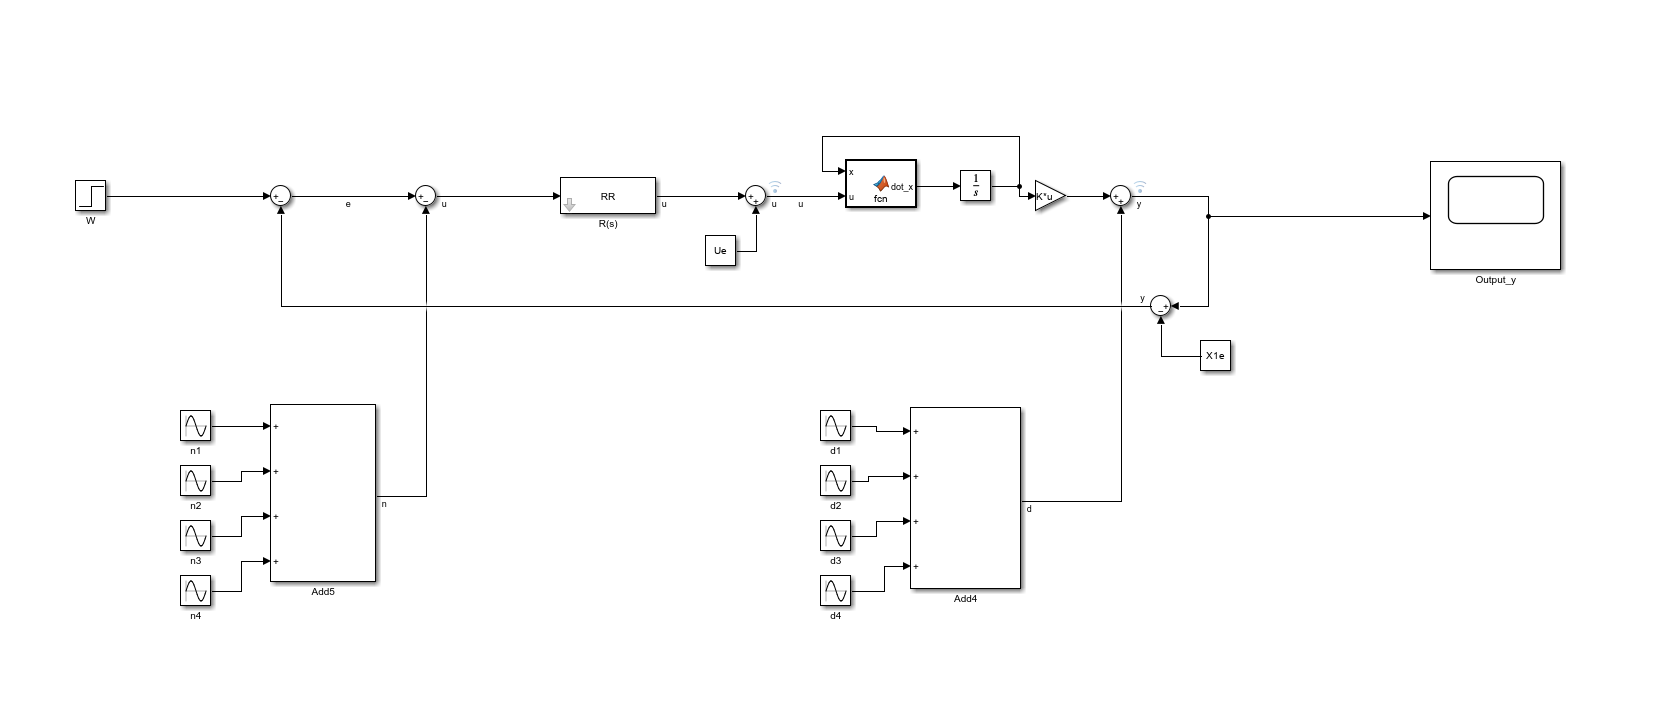
\includegraphics[width=110mm]{figs/simulink.PNG}
    \caption{}
    \label{Figura9}
\end{figure}

In figura mostreremo l'uscita del sistema non lineare considerando $n(t)$ e $d(t)$.
\begin{figure}[H]
    \centering
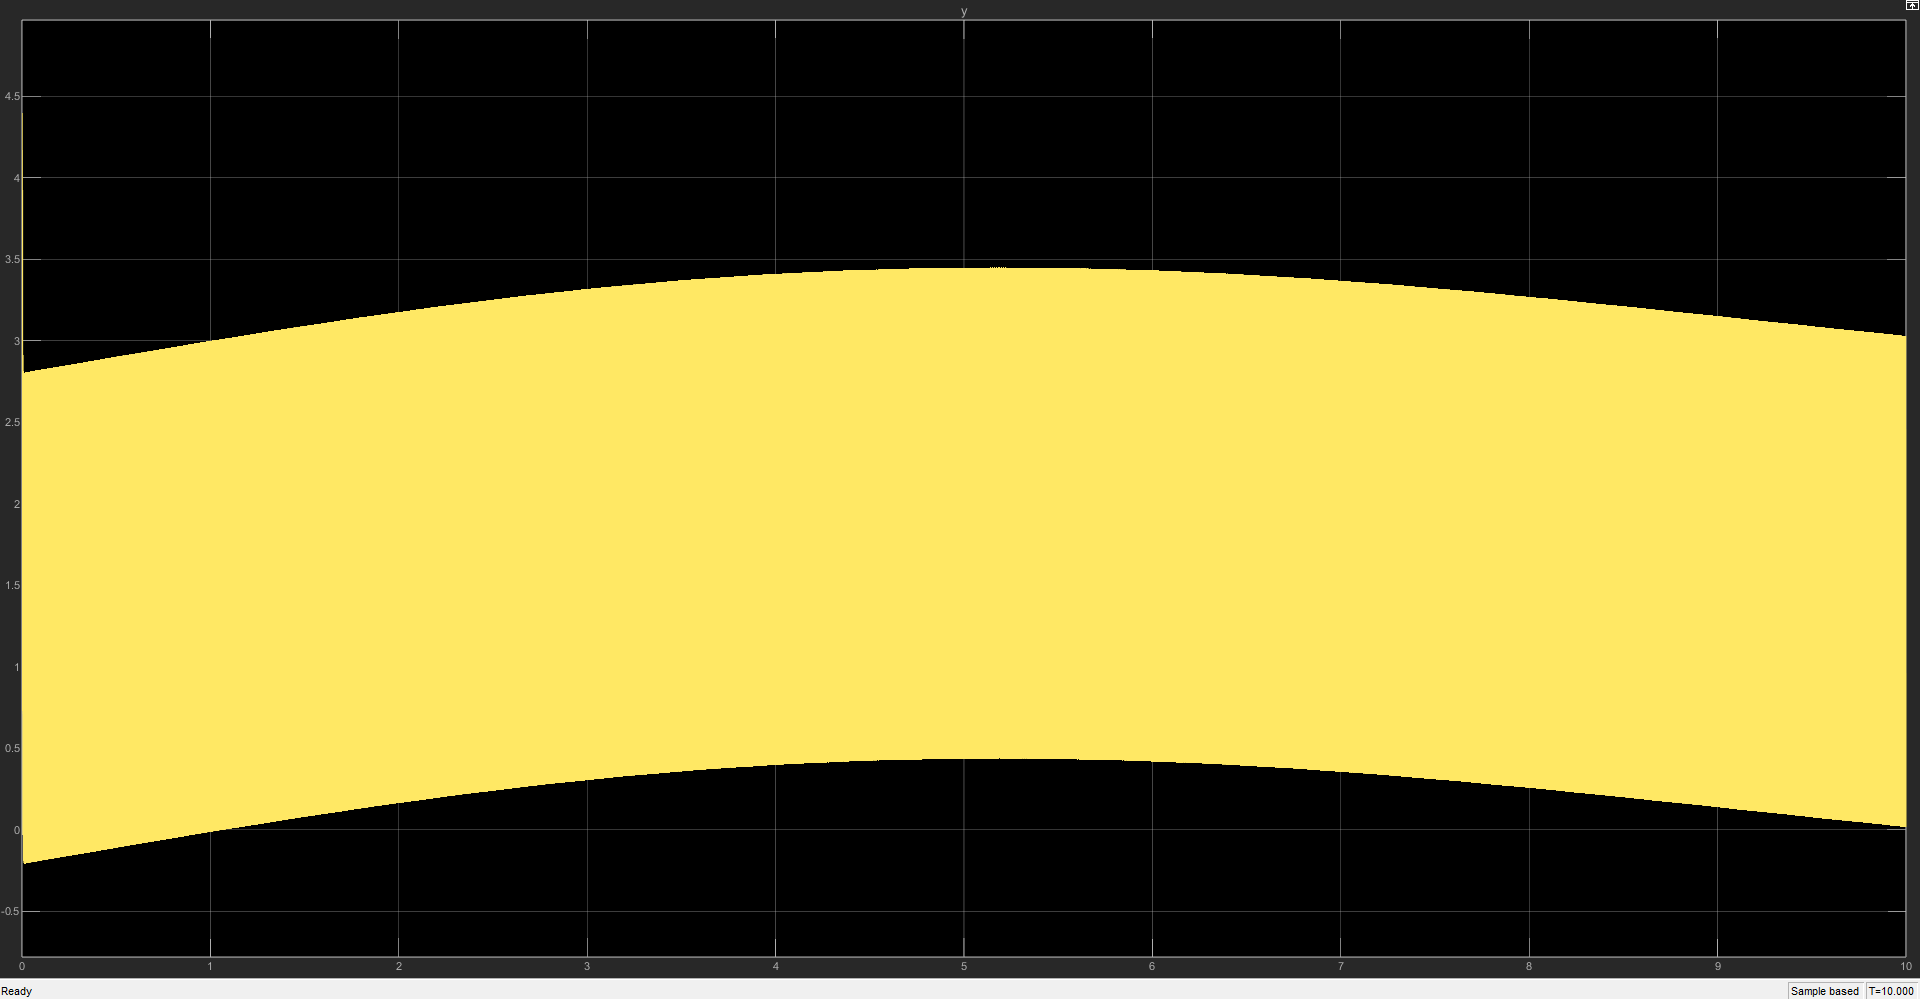
\includegraphics[width=110mm]{figs/nonLineare.PNG}
    \caption{}
    \label{Figura10}
\end{figure}
\section{Sistema lineare e non lineare, conclusioni}

In conclusione, possiamo apprezzare come il sistema lineare in anello chiuso rispetti le specifiche assegnate e, una volta esaurito il transitorio, l'uscita tenda a seguire il riferimento w(t) assegnato. Il sistema non lineare, invece, mostra che il regolatore si comporta diversamente rispetto alle specifiche. Questo accade perché il sistema non è predisposto alla linearizzazione o, comunque, presenta un'elevata imprecisione rispetto al sistema originale, che causa tale comportamento indesiderato.

\section{Punto opzionale: range di condizioni iniziali}

Supponendo un riferimento w(t) ≡ 0, esploriamo il range di condizioni iniziali dello stato del sistema non lineare (nell’intorno del punto di equilibrio) tali per cui l’uscita del sistema in anello chiuso converga a h(xe,ue).

Per fare ciò, riprendiamo il modello non lineare del sistema su simulink e alteriamo le condizioni iniziali del componente di integrazione. In particolare aggiungiamo ad entrambe le componenti di equilibrio $\theta_e$ e $\omega_e$ una \delta che faremo variare a nostro piacimento fino a trovare il range di condizioni iniziali che ci permettono di convergere all'uscita desiderata.
Inoltre per poter ottenere dei grafici leggibili e avere una effetiva convergenza, abbiamo deciso di togliere il rumore e il disturbo dal sistema.
Riportiamo in seguito i grafici ottenuti con simulink.

\begin{figure}[H]
    \centering
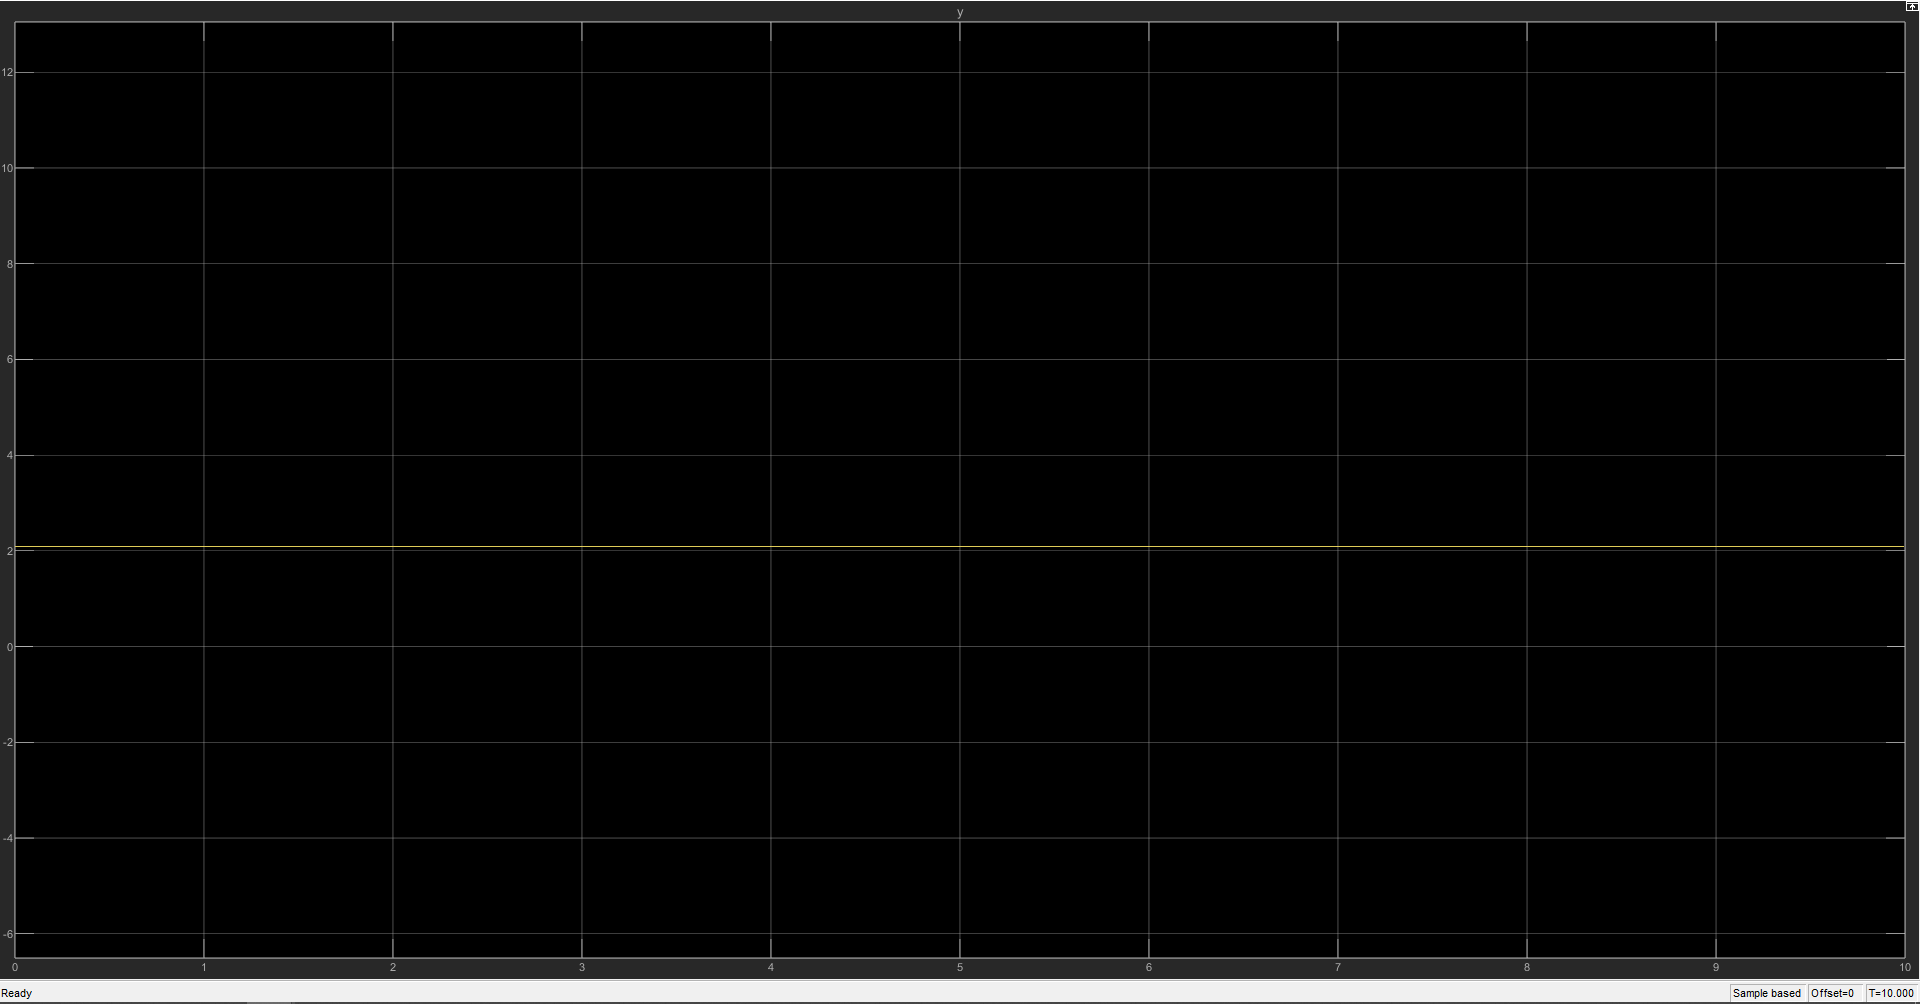
\includegraphics[width=110mm]{figs/delta0.PNG}
    \caption{}
    \label{Figura11: delta = 0}
\end{figure}

\begin{figure}[H]
    \centering
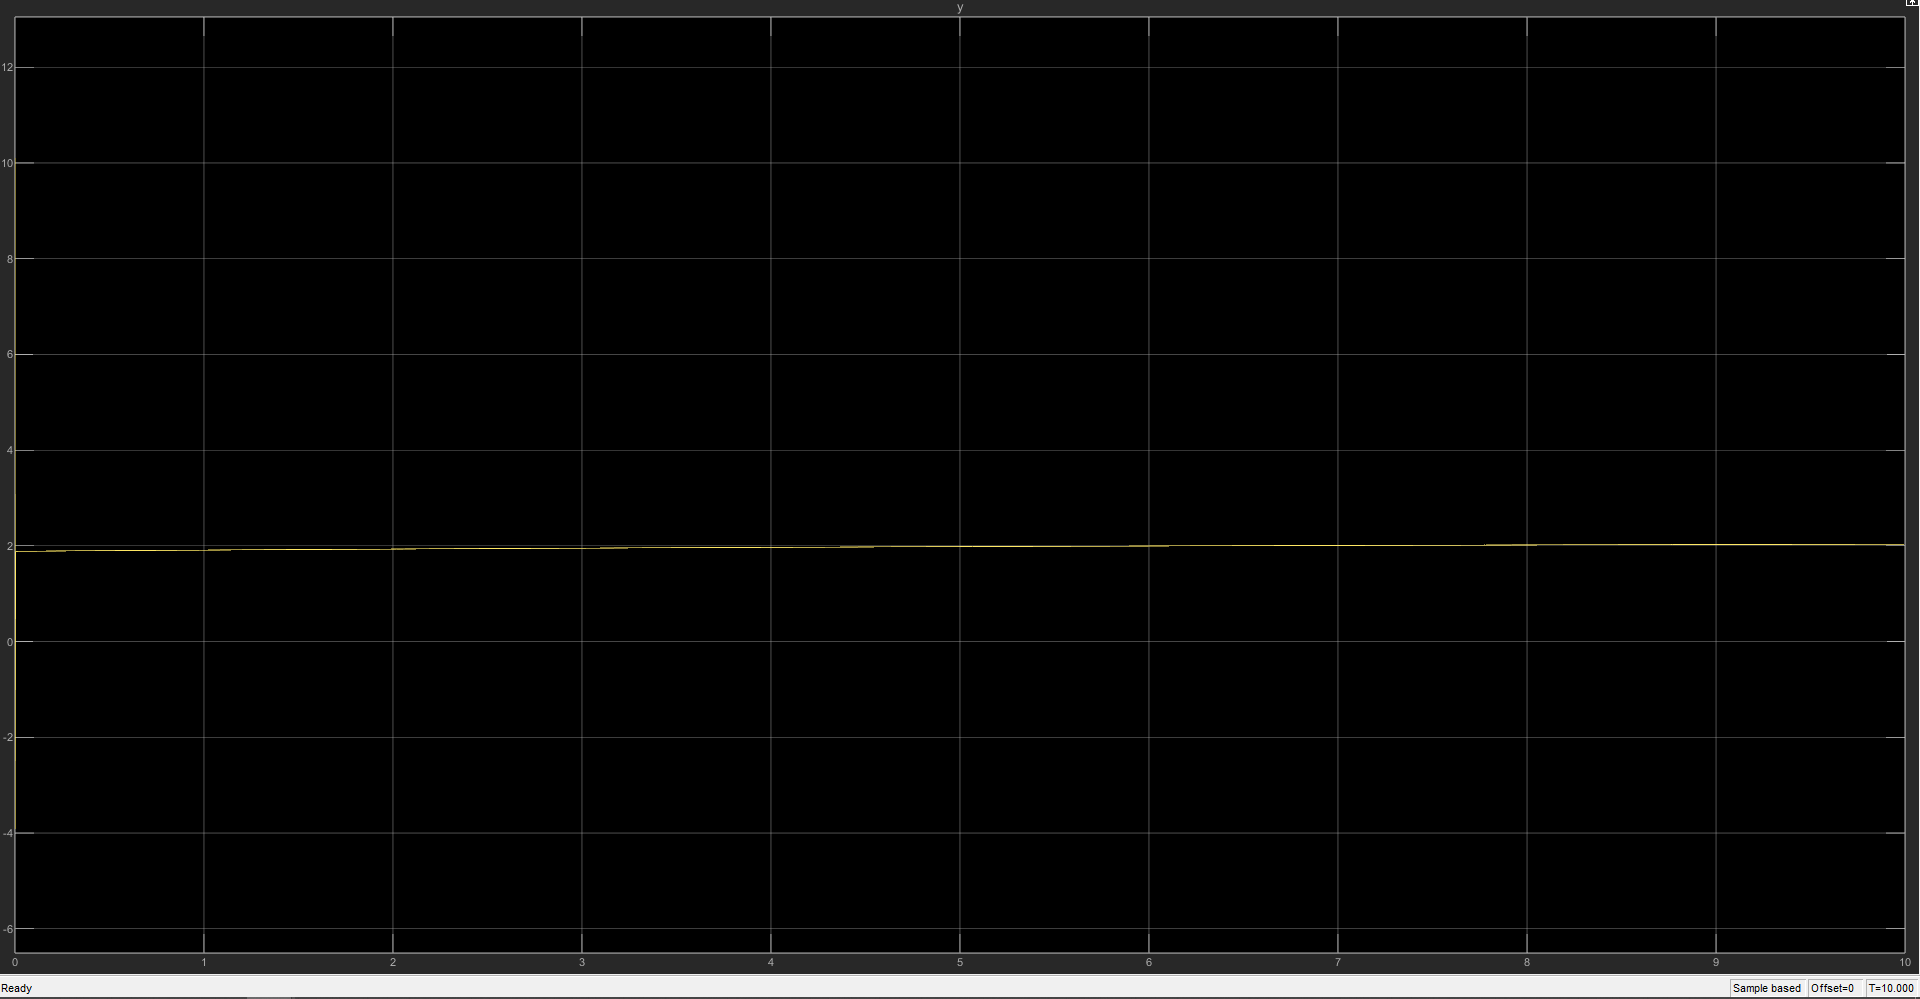
\includegraphics[width=110mm]{figs/delta8.PNG}
    \caption{}
    \label{Figura10: delta = 8}
\end{figure}

\begin{figure}[H]
    \centering
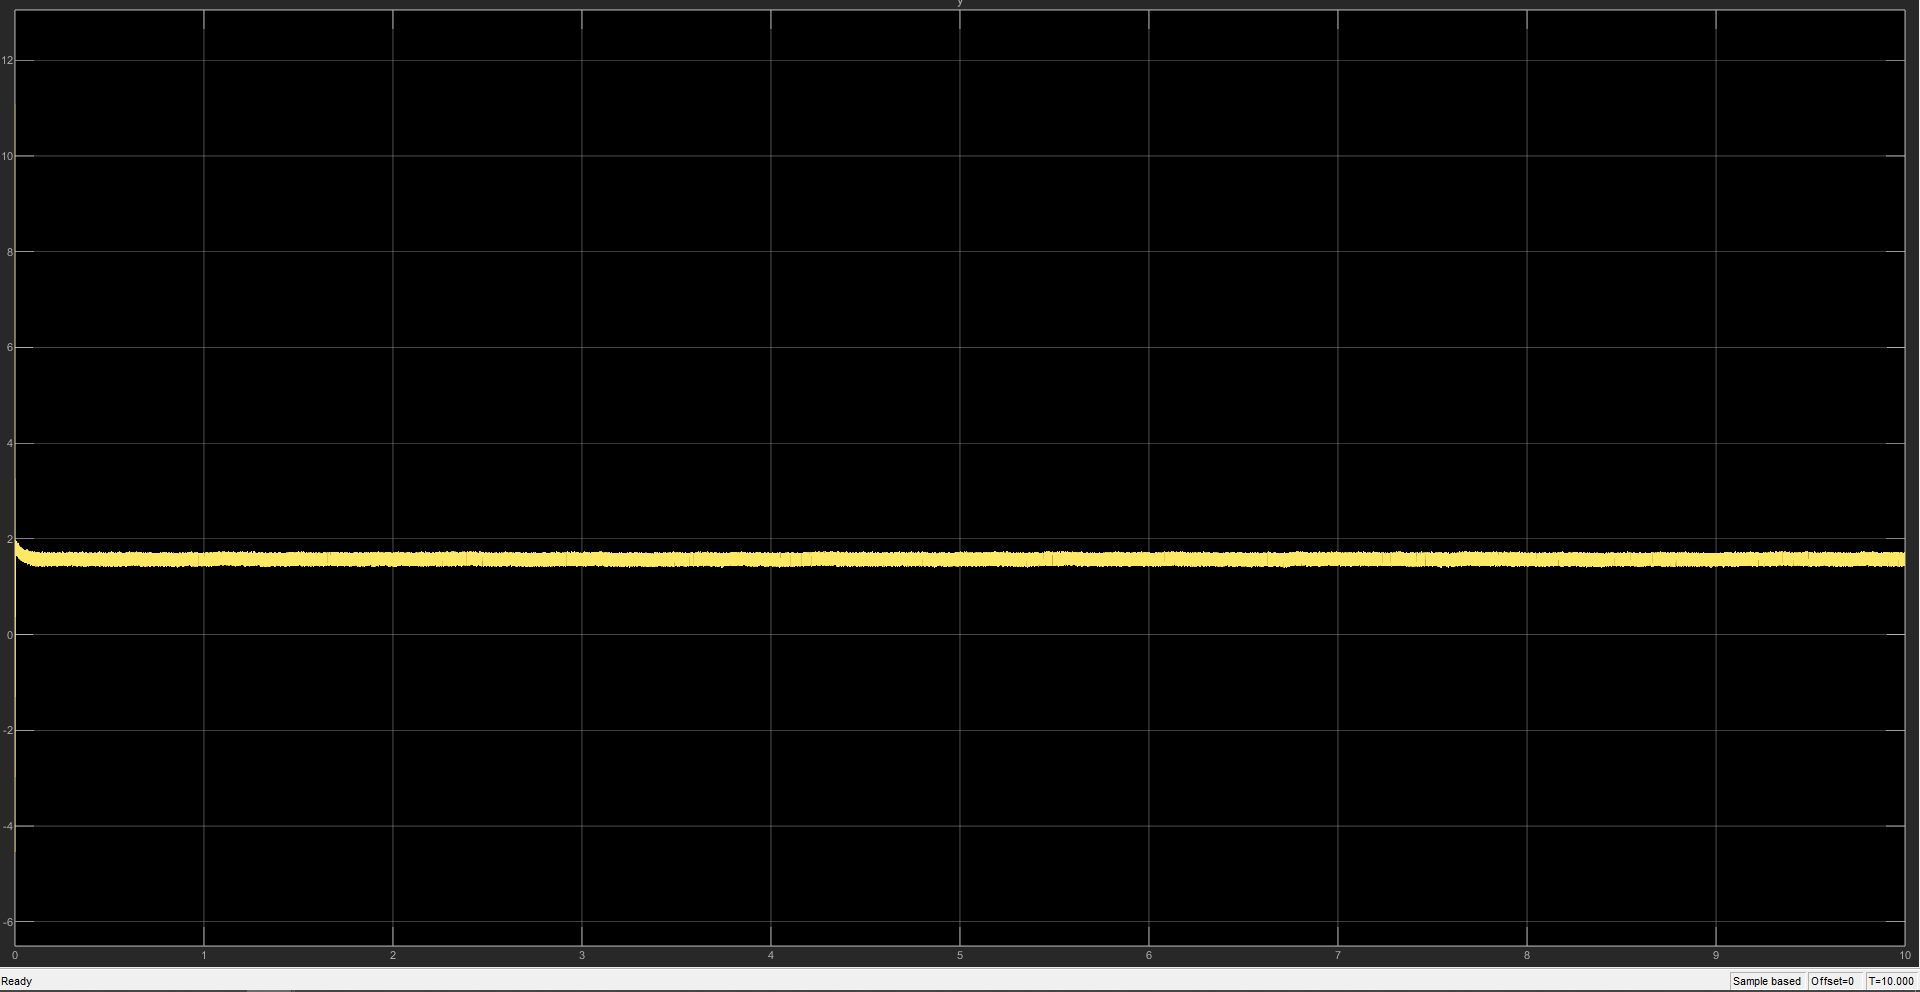
\includegraphics[width=110mm]{figs/delta9.PNG}
    \caption{}
    \label{Figura10: delta = 9}
\end{figure}

\section{Conclusione punto opzionale}
Possiamo notare che per valori di $\delta$ compresi tra 0 e 8 l'uscita del sistema non lineare converge a $h(xe,ue)$, mentre per valori di $\delta$ maggiori di 8 l'uscita del sistema non lineare non converge verso $h(xe,ue)$.

\end{document}
